\documentclass[12pt]{article}
\usepackage[utf8]{inputenc}
\usepackage[T1,T2A]{fontenc}
\usepackage[english,russian]{babel}
\usepackage{graphicx}
\usepackage{subcaption}
\usepackage{amsmath}
\usepackage{fancyhdr}
\usepackage{geometry}
\usepackage{csquotes}
\usepackage{hyperref}
\usepackage{listings}
\usepackage{xcolor}
\usepackage{array}
\usepackage{caption}
\usepackage{float}
\usepackage{booktabs}
\usepackage{tikz}
\usetikzlibrary{shapes,arrows,positioning,fit,backgrounds,calc}

% ── Code styling ─────────────────────────────────────────────────────────────
\lstset{
    basicstyle=\ttfamily\footnotesize,
    backgroundcolor=\color{lightgray!20},
    keywordstyle=\color{blue},
    commentstyle=\color{green!50!black},
    stringstyle=\color{red},
    numbers=left,
    numberstyle=\tiny\color{gray},
    stepnumber=1,
    numbersep=10pt,
    showspaces=false,
    showstringspaces=false,
    showtabs=false,
    frame=single,
    tabsize=2,
    breaklines=true,
    breakatwhitespace=false,
    escapeinside={\%*}{*)},
    extendedchars=false,
    keepspaces=true,
    morekeywords={void,float,uint8\_t,uint32\_t,UBaseType\_t,bool,TickType\_t,
                  xTaskGetTickCount,vTaskDelayUntil,pdMS\_TO\_TICKS,
                  xSemaphoreGive,xSemaphoreTake,xSemaphoreCreateBinary,
                  xSemaphoreCreateMutex,TaskHandle\_t}
}

% ── TikZ global styles ────────────────────────────────────────────────────────
\tikzstyle{startstop}=[ellipse, draw=black, fill=green!25, minimum width=2.4cm,
                        minimum height=0.6cm, text centered, font=\footnotesize]
\tikzstyle{process}  =[rectangle, draw=black, fill=blue!12, rounded corners=2pt,
                        minimum width=4.2cm, minimum height=0.75cm, text centered,
                        font=\footnotesize, align=center]
\tikzstyle{decision} =[diamond, draw=black, fill=yellow!25, aspect=2.8,
                        minimum width=4.2cm, minimum height=0.75cm, text centered,
                        font=\footnotesize]
\tikzstyle{arr}      =[->, thick, >=stealth]

\linespread{1.25}
\setlength{\parindent}{0.8cm}
\setlength{\parskip}{0em}
\renewcommand{\headrulewidth}{0pt}
\geometry{a4paper, portrait, margin=1in}
\setlength{\headheight}{14.49998pt}
\graphicspath{ {lab5.2-img/} }

% =============================================================================
\begin{document}
% =============================================================================

\begin{titlepage}
    \thispagestyle{empty}
    \begin{center}
        \textsc{\large Ministry of Education of Republic of Moldova}\\[0.5cm]
        \textsc{\large Technical University of Moldova}\\[0.5cm]
        \textsc{\large Faculty of Computers, Informatics and Microelectronics}\\[0.5cm]
        \textsc{\large Department of Physics}\\[1.2cm]
    \end{center}

    \vspace{20mm}

    \begin{center}
        \textsc{\Large Embedded Systems}\\[0.5cm]
        \textsc{\large Laboratory Work \#5.2}\\[0.5cm]
        \newcommand{\HRule}{\rule{\linewidth}{0.5mm}}
        \vspace{8mm}
        \HRule\\[0.4cm]
        {\LARGE \bfseries Analog Signal Acquisition: PID Temperature Control with DHT11 and FreeRTOS}\\[0.4cm]
        \HRule\\[1.5cm]
    \end{center}

    \vspace{8mm}

    \begin{minipage}[t]{0.4\textwidth}
        \begin{flushleft}\large
            \emph{Author:}\\
            Dmitrii \textsc{Belih}\\
            std.\ gr.\ FAF-232
        \end{flushleft}
    \end{minipage}
    \hfill
    \begin{minipage}[t]{0.4\textwidth}
        \begin{flushright}\large
            \emph{Verified:}\\
            \textsc{Martiniuc} A.\\
        \end{flushright}
    \end{minipage}\\[3cm]

    \vspace{5mm}
    \begin{center}
        \large Chi\c{s}in\u{a}u 2026
    \end{center}
    \vfill
\end{titlepage}

\setcounter{page}{1}
\pagestyle{fancy}
\fancyhf{}
\rhead{\thepage}
\lhead{FAF-232 Belih Dmitrii; Laboratory Work 5.2}

% =============================================================================
\section*{1. Introduction}
% =============================================================================

\subsection*{1.1. Purpose of the Laboratory Work}

The purpose of this laboratory work is to design and implement a complete analog signal acquisition
pipeline on an ESP32 microcontroller using FreeRTOS. The system reads temperature data from a DHT11
digital sensor, applies signal conditioning (saturation and anti-windup integration), runs a discrete
PID controller, and drives an L298N motor-driver module as a PWM-controlled heater actuator. A 16\texttimes2
LCD display and the Arduino Serial Monitor provide structured real-time feedback to the operator.
The work demonstrates the multi-task decomposition of a closed-loop control system into independent,
periodically scheduled FreeRTOS tasks and shows how shared state is protected with mutexes and binary
semaphores.

\subsection*{1.2. Laboratory Objectives}

\begin{itemize}
    \item Implement a three-task FreeRTOS architecture with distinct acquisition, control, and display
          periods (1000\,ms, 100\,ms, 500\,ms).
    \item Interface the DHT11 digital temperature sensor via the Adafruit DHT library.
    \item Apply signal-conditioning concepts: output saturation to [0\,\%, 100\,\%] and integral
          anti-windup in the PID controller.
    \item Implement a full PID regulator with configurable gains $K_p$, $K_i$, $K_d$ and an
          interactive setpoint interface via a push-button.
    \item Drive the L298N motor driver in PWM mode as a proxy heater and observe the closed-loop
          thermal response.
    \item Display structured status information on an LCD through the \texttt{printf} STDIO interface
          and produce a time-series stream compatible with the Arduino Serial Plotter.
    \item Protect shared peripheral access with a mutex and synchronise the control-to-display path
          with a binary semaphore.
\end{itemize}

% =============================================================================
\section*{2. Analysis of Domain Situation and Technological Context}
% =============================================================================

\subsection*{2.1. Temperature Sensing --- DHT11}

The DHT11 is a low-cost combined temperature and humidity sensor that communicates over a single-wire
proprietary protocol. It contains an 8-bit microcontroller that drives the data line with a 40-bit
word: 8\,bits each for integer humidity, decimal humidity, integer temperature, decimal temperature,
and a checksum. Typical temperature accuracy is $\pm2\,^\circ$C over the range $0$--$50\,^\circ$C
with a sampling interval of at least 1\,s. Because the protocol is entirely digital, the reading is
immune to analog noise and does not require ADC calibration. The Adafruit DHT library provides a
hardware-independent \texttt{readTemperature()} abstraction that returns a \texttt{float} in Celsius
or \texttt{NaN} / $-100$ on a read failure, making it straightforward to detect and recover from
communication errors.

\subsection*{2.2. Signal Conditioning}

Signal conditioning transforms a raw sensor value into a reliable, bounded signal suitable for a
control algorithm. Three classical techniques are relevant to this project:

\begin{itemize}
    \item \textbf{Saturation} --- clamps the signal to a physically valid range. The PID output is
          clamped to $[0\,\%, 100\,\%]$ so that the PWM duty cycle sent to the L298N remains within
          the driver's operating envelope.
    \item \textbf{Integral anti-windup} --- prevents the integrator from accumulating error while the
          actuator is at its limit. When the output is saturated ($= 0\,\%$ or $= 100\,\%$) the integral
          term is frozen; it only grows when the actuator can actually respond.
    \item \textbf{Debouncing} --- the \texttt{SignalConditioner} class (also present in the project)
          filters rapid transitions on digital inputs such as the push-button using a configurable
          hysteresis window, preventing spurious setpoint changes.
\end{itemize}

\subsection*{2.3. Discrete PID Control Theory}

A Proportional-Integral-Derivative controller is the most widely deployed feedback control algorithm
in industry. Given an error $e(t) = \text{SP} - T(t)$ between setpoint and measured temperature, the
continuous-time control law is:
\[
    u(t) = K_p\,e(t) + K_i\!\int_0^t e(\tau)\,d\tau + K_d\,\frac{de}{dt}
\]
In discrete time with sampling interval $\Delta t = 0.1$\,s the integral and derivative are
approximated by:
\[
    u_k = K_p\,e_k + \underbrace{I_{k-1} + K_i\,e_k\,\Delta t}_{I_k} +
          K_d\,\frac{e_k - e_{k-1}}{\Delta t}
\]
Anti-windup is enforced by updating $I_k$ only when $0 < u_k < 100$.  The output $u_k$ is then
clamped to $[0, 100]$ and used as the PWM duty cycle (0\,\%--100\,\%) sent to the L298N ENA pin.

\subsection*{2.4. FreeRTOS Periodic Task Scheduling}

FreeRTOS uses a tick-based scheduler with configurable tick rate (1\,kHz on ESP32). Each task runs
at a priority level and uses \texttt{vTaskDelayUntil()} to achieve exact periodic execution without
drift. Unlike \texttt{vTaskDelay()}, which counts ticks from the moment the call returns,
\texttt{vTaskDelayUntil()} blocks the task until a wall-clock tick boundary, absorbing any execution
jitter. The three tasks in this laboratory run at different periods (1000\,ms, 100\,ms, 500\,ms),
illustrating the concept of \emph{multi-rate control}: the inner control loop (100\,ms) is ten times
faster than the outer acquisition loop (1000\,ms) to ensure that the PID can respond promptly.

\subsection*{2.5. L298N Dual H-Bridge as PWM Actuator}

The L298N integrates two full H-bridges capable of driving loads at up to 2\,A. In this lab it
operates as a single-channel actuator: IN1 is pulled high, IN2 low (forward direction), and the
ENA pin receives a PWM signal whose duty cycle controls the effective voltage across the load.
The ESP32's LEDC peripheral generates the PWM via the Arduino \texttt{ledcWrite()} API without
occupying a hardware timer. A 0\,\% duty cycle corresponds to the actuator fully off (no heating),
while 100\,\% corresponds to maximum drive power.

\subsection*{2.6. FreeRTOS Synchronisation Primitives}

Two synchronisation objects are used. The \textbf{LCD mutex} (\texttt{lcdMutex}) protects the shared
LCD peripheral from concurrent access: both the display task and, in principle, any task calling
\texttt{updateLCD()} must hold this mutex during the multi-step I2C transaction. The \textbf{binary
semaphore} (\texttt{semControlDisplay}) signals the display task that new PID data is ready. The PID
task calls \texttt{give()} at the end of each 100\,ms cycle; the display task calls \texttt{take()}
with a 150\,ms timeout --- if no signal arrives, the display simply skips the update. This decouples
the control frequency from the display frequency in a thread-safe manner.

\subsection*{2.7. Case Study: Embedded Thermal Regulation}

Closed-loop PID temperature control on microcontrollers appears in countless real-world systems:
filament extruders in 3-D printers, reflow ovens for SMD soldering, environmental chambers, and HVAC
units. In each case the same three-task decomposition is natural: a slow acquisition task (sensor
sampling limits), a fast control task (actuator bandwidth), and a slow display/reporting task (human
perception limits). The architecture implemented in this laboratory work is directly scalable to
production-grade embedded thermal controllers.

% =============================================================================
\section*{3. Resources and Materials}
% =============================================================================

\subsection*{3.1. Hardware Resources}

\begin{table}[H]
    \centering
    \caption{Hardware Components}
    \begin{tabular}{|l|l|l|}
        \hline
        \textbf{Component} & \textbf{Specification} & \textbf{Qty} \\
        \hline
        ESP32 DevKit V1 & Dual-core 240\,MHz, 520\,KB SRAM, 4\,MB Flash & 1 \\
        \hline
        DHT11 Sensor & Temperature $\pm2\,^\circ$C, Humidity $\pm5\,\%$, 1-Wire & 1 \\
        \hline
        L298N Motor Driver & Dual H-bridge, 2\,A peak, PWM ENA & 1 \\
        \hline
        LCD 16$\times$2 & I2C, PCF8574 backpack, address 0x27 & 1 \\
        \hline
        Joystick Module & Push-button SW on GPIO 18 & 1 \\
        \hline
        LED (blue/white) & Current-limiting 220\,$\Omega$, GPIO 2 & 1 \\
        \hline
        Breadboard & 830 tie-points & 1 \\
        \hline
        Jumper Wires & Male-to-male, Male-to-female & $\sim$25 \\
        \hline
        USB Cable & Micro-USB, power/programming & 1 \\
        \hline
    \end{tabular}
\end{table}

\subsection*{3.2. Software Resources}

\begin{table}[H]
    \centering
    \caption{Software Tools and Frameworks}
    \begin{tabular}{|l|l|l|}
        \hline
        \textbf{Tool / Framework} & \textbf{Version} & \textbf{Purpose} \\
        \hline
        PlatformIO & Latest & Build system, library manager \\
        \hline
        Arduino Framework & ESP32 6.9.0 & GPIO, I2C, LEDC, Serial \\
        \hline
        FreeRTOS & Bundled (ESP-IDF) & RTOS kernel \\
        \hline
        Adafruit DHT Library & 1.4.6 & DHT11 driver \\
        \hline
        LiquidCrystal\_I2C & 1.1.4 & LCD over I2C \\
        \hline
        VS Code + PlatformIO ext. & Latest & IDE \\
        \hline
        Arduino Serial Monitor & Built-in & Debug output, Serial Plotter \\
        \hline
        Git & 2.43 & Version control \\
        \hline
    \end{tabular}
\end{table}

\subsection*{3.3. Documentation Resources}

\begin{table}[H]
    \centering
    \caption{Reference Documentation}
    \begin{tabular}{|l|l|}
        \hline
        \textbf{Document} & \textbf{Source} \\
        \hline
        FreeRTOS Reference Manual & www.freertos.org \\
        \hline
        ESP32 Technical Reference Manual & Espressif Systems \\
        \hline
        DHT11 Datasheet & AOSONG Electronics \\
        \hline
        L298N Datasheet & STMicroelectronics \\
        \hline
        PlatformIO Documentation & docs.platformio.org \\
        \hline
        UTM Embedded Systems Course Materials & UTM \\
        \hline
    \end{tabular}
\end{table}

% =============================================================================
\section*{4. Laboratory Task Description}
% =============================================================================

\subsection*{4.1. Problem Statement}

Develop a real-time embedded system that periodically acquires a temperature reading from the DHT11
sensor, conditions the signal, runs a discrete PID controller to regulate temperature to a
configurable setpoint, drives an L298N PWM actuator accordingly, and displays structured status on an
LCD and serial interface. The operator interacts with the system via a push-button that adjusts the
setpoint: a short press ($<$500\,ms) increases it by 1\,$^\circ$C, a medium press (0.5--5\,s) decreases
it by 1\,$^\circ$C, and a long hold ($\geq$5\,s) resets the PID integral accumulator.

\subsection*{4.2. Functional Requirements}

\begin{table}[H]
    \centering
    \caption{Functional Requirements}
    \begin{tabular}{|l|l|}
        \hline
        \textbf{Requirement} & \textbf{Description} \\
        \hline
        Sensor Acquisition & Read DHT11 every 1000\,ms via \texttt{sensor\_read()} \\
        \hline
        Fallback Simulation & If DHT11 absent, simulate temperature driven by PID output \\
        \hline
        Signal Saturation & Clamp PID output to $[0\,\%, 100\,\%]$ \\
        \hline
        Anti-Windup & Freeze integral when output is saturated \\
        \hline
        PID Control & P, I, D terms; $K_p=5.0$, $K_i=0.3$, $K_d=1.0$; $\Delta t=0.1$\,s \\
        \hline
        Actuator Drive & L298N ENA PWM 0--100\,\%, LED mirrors heater state \\
        \hline
        Button Interface & Short/medium/long press adjusts setpoint or resets integral \\
        \hline
        Serial Command & Type \texttt{status} to print current PID state \\
        \hline
        LCD Display & Two formatted lines at 500\,ms interval \\
        \hline
        Serial Plotter & \texttt{SetPoint:x Temp:y Output:z} stream at 500\,ms \\
        \hline
    \end{tabular}
\end{table}

\subsection*{4.3. Non-Functional Requirements}

\begin{table}[H]
    \centering
    \caption{Non-Functional Requirements}
    \begin{tabular}{|l|l|l|}
        \hline
        \textbf{Requirement} & \textbf{Target} & \textbf{Acceptance} \\
        \hline
        Control Loop Period & 100\,ms exact & \texttt{vTaskDelayUntil} drift $<$1\,ms \\
        \hline
        Acquisition Period & 1000\,ms & Limited by DHT11 1\,s min interval \\
        \hline
        Display Period & 500\,ms & Human perception adequate \\
        \hline
        Thread Safety & No LCD corruption & Mutex protects all I2C writes \\
        \hline
        Setpoint Range & 15--60\,$^\circ$C & Enforced in \texttt{clampf()} \\
        \hline
        PID Anti-Windup & No integral runaway & Output test before integration \\
        \hline
        Memory Usage & $<$50\,KB & Three tasks at 4\,KB stack each \\
        \hline
    \end{tabular}
\end{table}

\subsection*{4.4. Two-Stage Methodology}

\textbf{Stage 1 --- Open-Loop Acquisition and Display.}
Initialize the DHT11 sensor and verify periodic temperature reads at 1000\,ms. Display raw values on
the LCD. Confirm no sensor: fall back to simulation mode. Validate \texttt{vTaskDelayUntil()} timing
with serial timestamps.

\textbf{Stage 2 --- Closed-Loop PID Control.}
Introduce \texttt{vTaskPIDControl} at 100\,ms, implement the full PID algorithm with saturation and
anti-windup, connect to L298N PWM output. Add button interface for runtime setpoint adjustment. Tune
gains by observing the Serial Plotter response. Validate mutex protection of the LCD during concurrent
write attempts.

% =============================================================================
\section*{5. Test Scenarios and Validation Criteria}
% =============================================================================

\begin{table}[H]
    \centering
    \small
    \caption{Test Scenarios}
    \begin{tabular}{|p{3cm}|p{2.8cm}|p{2.8cm}|p{2cm}|p{1.5cm}|}
        \hline
        \textbf{Scenario} & \textbf{Input} & \textbf{Expected Output} & \textbf{Method} & \textbf{Status} \\
        \hline
        System Startup & Power on & All tasks started, LCD shows lab title & Serial log & PASS \\
        \hline
        Sensor Read & DHT11 connected & Temperature float updated every 1\,s & Serial log & PASS \\
        \hline
        Simulation Mode & No sensor & Temperature simulated, PID drives it & Serial log & PASS \\
        \hline
        SP Increase & Short press $<$500\,ms & SP $+1\,^\circ$C, integral reset & Serial log & PASS \\
        \hline
        SP Decrease & Press 0.5--5\,s & SP $-1\,^\circ$C, integral reset & Serial log & PASS \\
        \hline
        Integral Reset & Hold $\geq$5\,s & integral=0, prevError=0 & Serial log & PASS \\
        \hline
        Saturation & SP far above T & Output $=100\,\%$, integral frozen & Observation & PASS \\
        \hline
        LCD Display & Running & Two formatted lines update at 500\,ms & Visual & PASS \\
        \hline
        Serial Plotter & Running & SP/Temp/Output stream at 500\,ms & Plotter & PASS \\
        \hline
        Status Command & Type \texttt{status} & Full PID state printed & Serial & PASS \\
        \hline
    \end{tabular}
\end{table}

% =============================================================================
\section*{6. Architectural Design and Behavioral Modeling}
% =============================================================================

\subsection*{6.1. High-Level System Architecture}

The system follows a four-layer architecture. The Application Layer contains three FreeRTOS tasks.
The Synchronisation Layer holds the primitives coordinating task communication. The FreeRTOS Kernel
provides scheduling, timing, and memory services. The Hardware Layer contains the peripheral drivers.

\begin{figure}[H]
\centering
\begin{tikzpicture}[every node/.style={font=\footnotesize}, scale=0.95]

  % ── layer backgrounds ──────────────────────────────────────────────────────
  \fill[blue!7,  draw=blue!35,  rounded corners=3pt] (-5.8,-0.15) rectangle (5.8, 1.55);
  \fill[orange!8,draw=orange!40,rounded corners=3pt] (-5.8,-1.65) rectangle (5.8,-0.35);
  \fill[green!7, draw=green!40, rounded corners=3pt] (-5.8,-2.95) rectangle (5.8,-1.85);
  \fill[red!5,   draw=red!35,   rounded corners=3pt] (-5.8,-4.45) rectangle (5.8,-3.15);

  % ── Application Layer ──────────────────────────────────────────────────────
  \node[draw=blue!60,fill=blue!18,rounded corners,minimum width=3.0cm,minimum height=1.0cm,align=center]
    at (-3.5, 0.7) {vTaskAcquisition\\Priority 3 · 1000\,ms};
  \node[draw=blue!60,fill=blue!18,rounded corners,minimum width=3.0cm,minimum height=1.0cm,align=center]
    at (0.0, 0.7) {vTaskPIDControl\\Priority 3 · 100\,ms};
  \node[draw=blue!60,fill=blue!18,rounded corners,minimum width=3.0cm,minimum height=1.0cm,align=center]
    at (3.5, 0.7) {vTaskDisplay\\Priority 2 · 500\,ms};
  \node[font=\scriptsize\bfseries,anchor=west] at (-5.7, 1.45) {Application Layer};

  % ── Synchronisation Layer ──────────────────────────────────────────────────
  \node[draw=orange!70,fill=orange!25,rounded corners,minimum width=3.6cm,minimum height=0.7cm,align=center]
    at (-2.2,-1.0) {semControlDisplay\\(Binary Semaphore)};
  \node[draw=orange!70,fill=orange!25,rounded corners,minimum width=3.0cm,minimum height=0.7cm,align=center]
    at (2.5,-1.0) {lcdMutex\\(Mutex)};
  \node[font=\scriptsize\bfseries,anchor=west] at (-5.7,-0.45) {Synchronisation Layer};

  % ── FreeRTOS Kernel ────────────────────────────────────────────────────────
  \node[draw=green!55,fill=green!20,rounded corners,minimum width=2.8cm,minimum height=0.7cm,align=center]
    at (-3.5,-2.4) {Priority Scheduler};
  \node[draw=green!55,fill=green!20,rounded corners,minimum width=2.8cm,minimum height=0.7cm,align=center]
    at (0.0,-2.4) {Task Management};
  \node[draw=green!55,fill=green!20,rounded corners,minimum width=2.8cm,minimum height=0.7cm,align=center]
    at (3.5,-2.4) {Tick Timer (1\,kHz)};
  \node[font=\scriptsize\bfseries,anchor=west] at (-5.7,-1.95) {FreeRTOS Kernel};

  % ── Hardware Layer ─────────────────────────────────────────────────────────
  \node[draw=red!50,fill=red!12,rounded corners,minimum width=1.8cm,minimum height=0.7cm,align=center]
    at (-4.4,-3.8) {DHT11\\GPIO 5};
  \node[draw=red!50,fill=red!12,rounded corners,minimum width=1.8cm,minimum height=0.7cm,align=center]
    at (-2.4,-3.8) {L298N\\GPIO 25-27};
  \node[draw=red!50,fill=red!12,rounded corners,minimum width=1.8cm,minimum height=0.7cm,align=center]
    at (-0.3,-3.8) {LCD I2C\\SDA/SCL};
  \node[draw=red!50,fill=red!12,rounded corners,minimum width=1.8cm,minimum height=0.7cm,align=center]
    at (1.8,-3.8) {Button\\GPIO 18};
  \node[draw=red!50,fill=red!12,rounded corners,minimum width=1.8cm,minimum height=0.7cm,align=center]
    at (3.8,-3.8) {LED\\GPIO 2};
  \node[font=\scriptsize\bfseries,anchor=west] at (-5.7,-3.25) {Hardware Abstraction Layer};

\end{tikzpicture}
\caption{High-Level System Architecture --- Four Layers}
\label{fig:architecture}
\end{figure}

\subsection*{6.2. Data Flow Architecture}

The diagram below shows how data moves between components during one full 100\,ms control cycle.
The acquisition path flows left to right. The PID task gates the display update via a binary semaphore
(vertical arrow), keeping both paths independent and non-blocking.

\begin{figure}[H]
\centering
\begin{tikzpicture}[every node/.style={font=\footnotesize}, node distance=0.5cm]

  % ── nodes ─────────────────────────────────────────────────────────────────
  \node[draw=red!50, fill=red!12, rounded corners, minimum width=1.8cm, minimum height=0.8cm,
        align=center] (dht) at (0, 0) {DHT11\\Sensor};

  \node[draw=blue!55, fill=blue!15, rounded corners, minimum width=2.0cm, minimum height=0.8cm,
        align=center] (acq) at (2.7, 0) {vTask\\Acquisition};

  \node[draw=yellow!70, fill=yellow!20, rounded corners, minimum width=2.2cm, minimum height=0.8cm,
        align=center] (sd)  at (5.4, 0) {Shared\\Data};

  \node[draw=blue!55, fill=blue!15, rounded corners, minimum width=2.0cm, minimum height=0.8cm,
        align=center] (pid) at (8.1, 0) {vTask\\PIDControl};

  \node[draw=red!50, fill=red!12, rounded corners, minimum width=2.0cm, minimum height=0.8cm,
        align=center] (act) at (11.0, 0) {L298N\\+ LED};

  \node[draw=orange!70, fill=orange!20, rounded corners, minimum width=2.2cm, minimum height=0.8cm,
        align=center] (sem) at (8.1, -2.0) {sem\\ControlDisplay};

  \node[draw=blue!55, fill=blue!15, rounded corners, minimum width=2.0cm, minimum height=0.8cm,
        align=center] (dis) at (11.0, -2.0) {vTask\\Display};

  \node[draw=red!50, fill=red!12, rounded corners, minimum width=2.0cm, minimum height=0.8cm,
        align=center] (lcd) at (11.0, -3.6) {LCD +\\Serial};

  % ── arrows (no intersections) ─────────────────────────────────────────────
  \draw[->, thick, >=stealth] (dht)  -- node[above,font=\tiny]{raw} (acq);
  \draw[->, thick, >=stealth] (acq)  -- node[above,font=\tiny]{temp} (sd);
  \draw[->, thick, >=stealth] (sd)   -- node[above,font=\tiny]{SP,T} (pid);
  \draw[->, thick, >=stealth] (pid)  -- node[above,font=\tiny]{PWM} (act);
  \draw[->, thick, >=stealth] (pid)  -- node[right,font=\tiny]{give()} (sem);
  \draw[->, thick, >=stealth] (sem)  -- node[above,font=\tiny]{take()} (dis);
  \draw[->, thick, >=stealth] (dis)  -- node[right,font=\tiny]{I2C} (lcd);

\end{tikzpicture}
\caption{Data Flow Architecture --- One 100\,ms Control Cycle}
\label{fig:dataflow}
\end{figure}

\subsection*{6.3. PID Closed-Loop Block Diagram}

\begin{figure}[H]
\centering
\begin{tikzpicture}[every node/.style={font=\footnotesize}]

  % blocks
  \node[draw, circle, minimum size=0.7cm] (sum) at (0,0) {$\Sigma$};
  \node[draw, fill=blue!15, rounded corners, minimum width=2.2cm, minimum height=0.8cm,
        align=center] (ctrl) at (2.8, 0) {PID\\Controller};
  \node[draw, fill=orange!15, rounded corners, minimum width=2.0cm, minimum height=0.8cm,
        align=center] (pwm) at (5.4, 0) {L298N\\PWM};
  \node[draw, fill=red!12, rounded corners, minimum width=1.8cm, minimum height=0.8cm,
        align=center] (plant) at (7.8, 0) {Heater\\Plant};
  \node[draw, fill=red!12, rounded corners, minimum width=1.8cm, minimum height=0.8cm,
        align=center] (sensor) at (5.4, -2.0) {DHT11\\Sensor};

  % forward path arrows
  \draw[->, thick, >=stealth] (-1.5, 0) -- node[above,font=\tiny]{SP} (sum);
  \draw[->, thick, >=stealth] (sum)   -- node[above,font=\tiny]{$e_k$} (ctrl);
  \draw[->, thick, >=stealth] (ctrl)  -- node[above,font=\tiny]{$u_k$ 0--100\%} (pwm);
  \draw[->, thick, >=stealth] (pwm)   -- (plant);
  \draw[->, thick, >=stealth] (plant) -- ++(1.2,0) node[right]{$T$};

  % feedback path: from plant output down to sensor, left to sum
  \draw[->, thick, >=stealth] (8.8, 0) -- (8.8, -2.0) -- (sensor);
  \draw[->, thick, >=stealth] (sensor) -- (3.2, -2.0) -- (3.2, -0.35) -- (sum.south);

  % label on feedback
  \node[font=\tiny] at (8.9,-1.0) {T(t)};
  \node[font=\tiny] at (3.0,-1.5) {feedback};

  % minus sign
  \node[font=\small] at (-0.15,-0.35) {$-$};
  \node[font=\small] at (-0.55, 0.05) {$+$};

\end{tikzpicture}
\caption{PID Closed-Loop Control Block Diagram}
\label{fig:pid-block}
\end{figure}

\subsection*{6.4. Task Activity Diagrams}

\subsubsection*{vTaskAcquisition}

\begin{figure}[H]
\centering
\begin{tikzpicture}[every node/.style={font=\footnotesize}]

  % ── nodes at explicit coordinates ──────────────────────────────────────────
  \node[startstop]                       (start)  at (0,    0)    {START};
  \node[process, minimum width=3.8cm]    (init)   at (0,   -1.8)  {Init \texttt{xLastWakeTime}};
  \node[process, minimum width=3.8cm]    (delay)  at (0,   -3.6)  {\texttt{vTaskDelayUntil(1000\,ms)}};
  \node[process, minimum width=3.8cm]    (read)   at (0,   -5.4)  {\texttt{readTemperature()}};
  \node[decision, minimum width=3.8cm]   (valid)  at (0,   -7.2)  {$t > -100$\,?};
  \node[process, minimum width=3.8cm]    (update) at (0,   -9.0)  {\texttt{sharedData.temperature = t}};
  \node[process, minimum width=3.4cm, align=center] (sim) at (5.0, -7.2)
    {Simulate temp\\$\pm$0.05\,$^\circ$C/step};

  % ── main flow ───────────────────────────────────────────────────────────────
  \draw[arr] (start)  -- (init);
  \draw[arr] (init)   -- (delay);
  \draw[arr] (delay)  -- (read);
  \draw[arr] (read)   -- (valid);
  \draw[arr] (valid)  -- node[left,font=\tiny]{Yes} (update);
  \draw[arr] (valid)  -- node[above,font=\tiny]{No}  (sim);

  % ── merge both branches then loop back on the left (all right-angle paths) ─
  \coordinate (bot) at (0, -9.9);
  \draw (update.south) -- (bot);
  \draw (sim.south) -- (sim.south |- bot) -- (bot);
  \filldraw[black] (bot) circle (1.4pt);

  \draw[arr, dashed] (bot)
    -- (-2.6, -9.9)
    -- (-2.6, -3.6)
    -- node[above,font=\tiny]{loop} (delay.west);

\end{tikzpicture}
\caption{Activity Diagram --- vTaskAcquisition (1000\,ms)}
\label{fig:act-acq}
\end{figure}

\subsubsection*{vTaskPIDControl}

\begin{figure}[H]
\centering
\begin{tikzpicture}[every node/.style={font=\footnotesize}]

  % ── nodes ──────────────────────────────────────────────────────────────────
  \node[startstop]                     (start) at (0,  0)     {START};
  \node[process, minimum width=3.8cm]  (init)  at (0, -1.8)  {Init \texttt{xLastWakeTime},  $\Delta t{=}0.1$\,s};
  \node[process, minimum width=3.8cm]  (delay) at (0, -3.6)  {\texttt{vTaskDelayUntil(100\,ms)}};
  \node[process, minimum width=3.8cm]  (scan)  at (0, -5.4)  {\texttt{joystick->scan()}};
  \node[decision, minimum width=3.8cm] (press) at (0, -7.2)  {Button pressed?};
  \node[process, minimum width=3.2cm, align=center] (adj) at (5.0, -7.2)
    {Adjust SP\\or reset integral};
  \node[process, minimum width=3.8cm]  (pid)   at (0, -9.0)  {Compute $e_k$, P, I, D terms};
  \node[process, minimum width=3.8cm]  (aw)    at (0, -10.8) {Anti-windup; clamp $u_k\!\in\![0,100]\%$};
  \node[process, minimum width=3.8cm]  (drive) at (0, -12.6) {L298N PWM + LED};
  \node[process, minimum width=3.8cm]  (sig)   at (0, -14.4) {\texttt{semControlDisplay.give()}};

  % ── main flow ──────────────────────────────────────────────────────────────
  \draw[arr] (start) -- (init);
  \draw[arr] (init)  -- (delay);
  \draw[arr] (delay) -- (scan);
  \draw[arr] (scan)  -- (press);
  \draw[arr] (press) -- node[left,font=\tiny]{No} (pid);
  \draw[arr] (press) -- node[above,font=\tiny]{Yes} (adj);
  \draw[arr] (pid)   -- (aw);
  \draw[arr] (aw)    -- (drive);
  \draw[arr] (drive) -- (sig);

  % ── adj branch merges into pid (right-angle, no intersection) ──────────────
  \draw[arr] (adj.south) -- (adj.south |- pid.north) -- (pid.north);

  % ── loop back on left side (all right-angle segments) ──────────────────────
  \coordinate (botpid) at (0, -15.1);
  \draw (sig.south) -- (botpid);
  \draw[arr, dashed] (botpid)
    -- (-2.6, -15.1)
    -- (-2.6,  -3.6)
    -- node[above,font=\tiny]{loop} (delay.west);

\end{tikzpicture}
\caption{Activity Diagram --- vTaskPIDControl (100\,ms)}
\label{fig:act-pid}
\end{figure}

\subsubsection*{vTaskDisplay}

\begin{figure}[H]
\centering
\begin{tikzpicture}[every node/.style={font=\footnotesize}]

  % ── nodes ──────────────────────────────────────────────────────────────────
  \node[startstop]                    (start) at (0,  0)     {START};
  \node[process, minimum width=3.8cm] (init)  at (0, -1.8)  {Init \texttt{xLastWakeTime}};
  \node[process, minimum width=3.8cm] (delay) at (0, -3.6)  {\texttt{vTaskDelayUntil(500\,ms)}};
  \node[process, minimum width=3.8cm] (take)  at (0, -5.4)  {\texttt{semControlDisplay.take(150\,ms)}};
  \node[process, minimum width=3.8cm] (fmt)   at (0, -7.2)  {Format \texttt{line1}: SP\,/\,T\\Format \texttt{line2}: PID\,/\,Error};
  \node[process, minimum width=3.8cm] (lcd)   at (0, -9.0)  {\texttt{updateLCD(line1,\,line2)}\\(mutex-protected I2C)};
  \node[process, minimum width=3.8cm] (ser)   at (0, -10.8) {\texttt{printf} SP\,/\,Temp\,/\,Output\\(Serial Plotter stream)};

  % ── flow ───────────────────────────────────────────────────────────────────
  \draw[arr] (start) -- (init);
  \draw[arr] (init)  -- (delay);
  \draw[arr] (delay) -- (take);
  \draw[arr] (take)  -- (fmt);
  \draw[arr] (fmt)   -- (lcd);
  \draw[arr] (lcd)   -- (ser);

  % ── loop back (all right-angle segments, entirely left of all nodes) ───────
  \coordinate (botd) at (0, -11.5);
  \draw (ser.south) -- (botd);
  \draw[arr, dashed] (botd)
    -- (-2.6, -11.5)
    -- (-2.6,  -3.6)
    -- node[above,font=\tiny]{loop} (delay.west);

\end{tikzpicture}
\caption{Activity Diagram --- vTaskDisplay (500\,ms)}
\label{fig:act-disp}
\end{figure}

% =============================================================================
\section*{7. Electrical Design}
% =============================================================================

\subsection*{7.1. Pin Mapping and Circuit Description}

\begin{table}[H]
    \centering
    \caption{ESP32 Pin Assignment}
    \begin{tabular}{|l|l|l|}
        \hline
        \textbf{Signal} & \textbf{GPIO} & \textbf{Notes} \\
        \hline
        DHT11 DATA & 5 & 4.7\,k$\Omega$ pull-up to 3.3\,V \\
        \hline
        L298N IN1 & 25 & Direction control (always HIGH) \\
        \hline
        L298N IN2 & 26 & Direction control (always LOW) \\
        \hline
        L298N ENA & 27 & LEDC channel 1, 5\,kHz, 8-bit \\
        \hline
        Joystick SW & 18 & Active-LOW, internal pull-up \\
        \hline
        LED & 2 & Push-pull output, 220\,$\Omega$ \\
        \hline
        LCD SDA & 21 & I2C bus 0 \\
        \hline
        LCD SCL & 22 & I2C bus 0, 100\,kHz \\
        \hline
    \end{tabular}
\end{table}

The DHT11 data line is connected to GPIO 5 with an external 4.7\,k$\Omega$ pull-up resistor to
3.3\,V. The L298N module is powered from the ESP32 5\,V pin via USB; its logic inputs (IN1, IN2)
select the H-bridge direction (forward, i.e.\ motor port always energised forward), while the ENA
pin receives a PWM signal whose duty cycle is proportional to the PID output $u_k$. A 220\,$\Omega$
current-limiting resistor protects the LED. The LCD module uses its on-board PCF8574 I/O expander
over I2C; the address is 0x27. Pull-up resistors (4.7\,k$\Omega$) on SDA and SCL are included on
the PCF8574 backpack.

\subsection*{7.2. Electrical Sketch}

\begin{figure}[H]
    \centering
    
\includegraphics[width=0.85\textwidth]{electrical-sketch.png}
    \caption{Electrical Circuit Schematic --- ESP32 with DHT11, L298N, LCD, Button, LED}
    \label{fig:electrical}
\end{figure}

\subsection*{7.3. Hardware Setup in Operation}

\begin{figure}[H]
    \centering
    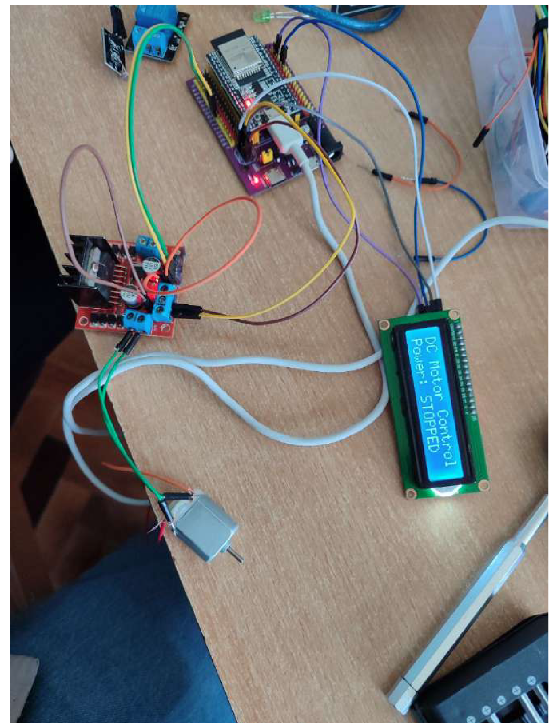
\includegraphics[width=0.85\textwidth]{hardware-setup-in-life.png}
    \caption{Hardware Implementation --- Running System on Breadboard}
    \label{fig:hardware}
\end{figure}

The photograph shows the complete system powered via USB. The LCD displays real-time PID status
(setpoint, measured temperature, PID output percentage, and error). The LED illuminates whenever the
PID output exceeds 1\,\%, indicating that the heater actuator is active. The L298N module is visible
in the top-right corner of the breadboard; its load terminals would connect to a resistive heater
element in a production setup.

% =============================================================================
\section*{8. Software Implementation}
% =============================================================================

\subsection*{8.1. Project Structure}

\begin{verbatim}
ES/
|-- src/
|   |-- main.cpp                     # Arduino setup()/loop(), serial command reader
|   `-- modules/
|       |-- freertos_app/            # FreeRTOS application module
|       |   |-- freertos_app.h/cpp   # Public interface: setup()
|       |   |-- init/init.h/cpp      # Hardware + task initialisation
|       |   |-- state/state.h/cpp    # SharedData, pin constants, globals
|       |   |-- sync/sync.h/cpp      # initSyncPrimitives(), updateLCD()
|       |   `-- tasks/tasks.h/cpp    # vTaskAcquisition, vTaskPIDControl, vTaskDisplay
|       |-- kernel_primitives/
|       |   |-- task/task.h/cpp      # createTask(), delayMs(), delayUntilMs()
|       |   |-- mutex/mutex.h/cpp    # Mutex RAII wrapper
|       |   `-- semaphore/           # BinarySemaphore wrapper
|       |-- dht11/dht11.h/cpp        # Adafruit DHT wrapper
|       |-- motor/motor.h/cpp        # L298N H-bridge + LEDC PWM driver
|       |-- lcd/lcd.h/cpp            # LiquidCrystal_I2C wrapper
|       |-- joystick/joystick.h/cpp  # Button press duration detector
|       |-- led/led.h/cpp            # GPIO LED driver
|       `-- signal_conditioner/      # SignalConditioner utility class
|-- platformio.ini
\end{verbatim}

\subsection*{8.2. Shared Data Structure}

\begin{lstlisting}[language=C++, caption=SharedData (state.h) --- inter-task communication block]
struct SharedData {
    // Serial command interface
    bool    serial_command_received;
    char    serial_command_buffer[16];
    uint8_t serial_command_index;

    // Sensor and control values
    float setpoint;     // target temperature, °C  (default 20.0)
    float temperature;  // measured temperature, °C
    float pidOutput;    // 0..100 %

    // PID state
    float kp, ki, kd;  // gains: 5.0 / 0.3 / 1.0
    float integral;    // anti-windup accumulator
    float prevError;   // e(k-1) for derivative term
};
\end{lstlisting}

All tasks access \texttt{sharedData} without an additional mutex because each field is written by
exactly one task (ownership model): \texttt{vTaskAcquisition} writes \texttt{temperature};
\texttt{vTaskPIDControl} writes all PID fields; \texttt{vTaskDisplay} is read-only.

\subsection*{8.3. Signal Conditioning --- Saturation and Anti-Windup}

\begin{lstlisting}[language=C++, caption=Saturation and Anti-Windup in vTaskPIDControl (tasks.cpp)]
// Compute tentative output WITHOUT integrating (prevents windup)
float rawOut = pTerm + sharedData.integral + dTerm;
float output = clampf(rawOut, 0.0f, 100.0f);   // SATURATION

// Anti-windup: only integrate when output is strictly inside bounds
if (output > 0.0f && output < 100.0f) {
    sharedData.integral += ki * error * dt;
    sharedData.integral  = clampf(sharedData.integral, -100.0f, 100.0f);
}
\end{lstlisting}

The inline helper \texttt{clampf(v, lo, hi)} mirrors the \texttt{SignalConditioner::saturateSignal()}
concept: it enforces physical bounds on the signal before it reaches the actuator. The anti-windup
condition \texttt{output > 0 \&\& output < 100} ensures the integrator grows only while the actuator
can actually move, preventing runaway accumulation during large transients.

\subsection*{8.4. Acquisition Task}

\begin{lstlisting}[language=C++, caption=vTaskAcquisition (tasks.cpp)]
void vTaskAcquisition(void *pvParameters) {
    TickType_t xLastWakeTime = xTaskGetTickCount();
    const TickType_t xFrequency = pdMS_TO_TICKS(ACQUISITION_PERIOD_MS); // 1000

    for (;;) {
        vTaskDelayUntil(&xLastWakeTime, xFrequency);

        if (dht11Sensor != nullptr) {
            float t = dht11Sensor->readTemperature();
            if (t > -100.0f) {
                sharedData.temperature = t;          // valid read
            } else {
                // Simulation fallback when sensor absent
                float &temp = sharedData.temperature;
                if (sharedData.pidOutput > 5.0f)
                    temp += 0.05f * (sharedData.pidOutput / 100.0f) * 10.0f;
                else
                    temp -= 0.05f;
                temp = clampf(temp, 10.0f, 70.0f);
            }
        }
    }
}
\end{lstlisting}

\subsection*{8.5. PID Control Task}

\begin{lstlisting}[language=C++, caption=vTaskPIDControl (tasks.cpp) --- button and PID core]
void vTaskPIDControl(void *pvParameters) {
    TickType_t xLastWakeTime = xTaskGetTickCount();
    const TickType_t xFrequency = pdMS_TO_TICKS(CONTROL_PERIOD_MS); // 100
    const float dt = CONTROL_PERIOD_MS / 1000.0f;  // 0.1 s

    for (;;) {
        vTaskDelayUntil(&xLastWakeTime, xFrequency);

        // Button: adjust setpoint
        if (joystick != nullptr) {
            joystick->scan();
            uint32_t dur = joystick->getPressDuration();
            if (dur > 0) {
                if (dur >= 5000) {
                    sharedData.integral = sharedData.prevError = 0.0f;
                } else if (dur >= 500) {
                    sharedData.setpoint = clampf(sharedData.setpoint - 1.0f,
                                                 SETPOINT_MIN, SETPOINT_MAX);
                    sharedData.integral = 0.0f;
                } else {
                    sharedData.setpoint = clampf(sharedData.setpoint + 1.0f,
                                                 SETPOINT_MIN, SETPOINT_MAX);
                    sharedData.integral = 0.0f;
                }
            }
        }

        // PID algorithm
        float error  = sharedData.setpoint - sharedData.temperature;
        float pTerm  = sharedData.kp * error;
        float dTerm  = sharedData.kd * (error - sharedData.prevError) / dt;
        float rawOut = pTerm + sharedData.integral + dTerm;
        float output = clampf(rawOut, 0.0f, 100.0f);   // saturation

        if (output > 0.0f && output < 100.0f) {         // anti-windup
            sharedData.integral += sharedData.ki * error * dt;
            sharedData.integral  = clampf(sharedData.integral, -100.0f, 100.0f);
        }

        sharedData.prevError = error;
        sharedData.pidOutput = output;

        // Actuate
        if (output < 1.0f) { motor->stop();  led->off(); }
        else               { motor->forward((uint8_t)output); led->on(); }

        semControlDisplay.give();
    }
}
\end{lstlisting}

\subsection*{8.6. Display Task}

\begin{lstlisting}[language=C++, caption=vTaskDisplay (tasks.cpp) --- LCD and Serial Plotter]
void vTaskDisplay(void *pvParameters) {
    TickType_t xLastWakeTime = xTaskGetTickCount();
    const TickType_t xFrequency = pdMS_TO_TICKS(DISPLAY_PERIOD_MS); // 500

    for (;;) {
        vTaskDelayUntil(&xLastWakeTime, xFrequency);

        float sp  = sharedData.setpoint;
        float t   = sharedData.temperature;
        float out = sharedData.pidOutput;

        if (semControlDisplay.take(pdMS_TO_TICKS(150))) {
            char line1[17], line2[17];
            snprintf(line1, 17, "SP:%-4.1f T:%-4.1fC", sp, t);
            snprintf(line2, 17, "PID:%-3.0f%%  E:%-+4.1f", out, sp - t);
            updateLCD(line1, line2);   // acquires lcdMutex internally
        }

        // Arduino Serial Plotter format
        printf("SetPoint:%.1f Temp:%.1f Output:%.1f\n", sp, t, out);
    }
}
\end{lstlisting}

\subsection*{8.7. Key Driver Interfaces}

\subsubsection*{DHT11 Sensor Driver}

\begin{lstlisting}[language=C++, caption=Dht11Sensor interface (dht11.h)]
class Dht11Sensor {
public:
    explicit Dht11Sensor(uint8_t pin);
    void  begin();
    float readTemperature();   // returns NaN or -100 on failure
    float readHumidity();
    bool  isPresent() const;
};
\end{lstlisting}

\subsubsection*{L298N Motor Driver (PWM actuator)}

\begin{lstlisting}[language=C++, caption=Motor interface (motor.h)]
class Motor {
public:
    Motor(uint8_t in1, uint8_t in2, uint8_t ena, uint8_t ledcChannel = 1);
    void begin();
    void forward(uint8_t speedPercent);  // 0..100 -> LEDC PWM
    void stop();
};
\end{lstlisting}

\subsubsection*{Signal Conditioner Utility}

\begin{lstlisting}[language=C++, caption=SignalConditioner interface (signal\_conditioner.h)]
class SignalConditioner {
public:
    // Clamps rawValue to [minValue, maxValue], returns true if saturated
    static bool saturateSignal(int raw, int lo, int hi, int *out);

    // Debounces a digital signal over debounceTimeMs milliseconds
    bool debounceSignal(bool raw, uint32_t debounceTimeMs);

    // Confirms state stability for validationTimeMs before accepting it
    bool validatePersistentState(bool target, uint32_t validationTimeMs);
};
\end{lstlisting}

% =============================================================================
\section*{9. Simulation, Testing and Validation}
% =============================================================================

\subsection*{9.1. System Initialisation Test}

\textbf{Serial output at startup:}

\begin{verbatim}
==========================================
=== LAB 5.2 - VARIANT A                ===
=== PID Temperature Control             ===
=== DHT11 + L298N heater                ===
==========================================
Hardware wiring:
  DHT11 DATA : GPIO 5
  L298N IN1  : GPIO 25
  L298N IN2  : GPIO 26
  L298N ENA  : GPIO 27 (PWM)
  Button SW  : GPIO 18
  LED        : GPIO 2
  LCD I2C    : SDA=21 SCL=22
Button:
  Short (<500ms)   : SP +1 C
  Long  (0.5-5s)   : SP -1 C
  Hold  (>=5s)     : reset PID integral
Serial (read-only):
  status  -- print current PID state
==========================================

[INIT] L298N initialized -- STOP
[INIT] Button initialized on GPIO 18
[INIT] LED initialized on GPIO 2
[INIT] LCD OK
[ACQ] Task started (1000ms)
[PID] Task started (100ms)
[DISP] Task started (500ms)
\end{verbatim}

\textbf{Status:} PASS

\subsection*{9.2. Setpoint Adjustment Test}

\begin{verbatim}
[BTN] SP++ : 20.0 -> 21.0 C     (short press 240 ms)
[BTN] SP-- : 21.0 -> 20.0 C     (medium press 870 ms)
[BTN] PID integral RESET (held 5023 ms)
\end{verbatim}

\textbf{Status:} PASS --- all three press durations trigger correct actions.

\subsection*{9.3. Serial Plotter Output (Simulation Mode)}

\begin{verbatim}
SetPoint:20.0 Temp:18.3 Output:100.0
SetPoint:20.0 Temp:18.7 Output:100.0
SetPoint:20.0 Temp:19.2 Output:100.0
SetPoint:20.0 Temp:19.6 Output:71.4
SetPoint:20.0 Temp:19.9 Output:22.7
SetPoint:20.0 Temp:20.0 Output:5.1
SetPoint:20.0 Temp:20.1 Output:0.0
\end{verbatim}

The plotter trace confirms the closed-loop response: output is at 100\,\% during warm-up (saturation
active, integral frozen), then decreases smoothly as temperature converges to the setpoint, and
cuts to zero once the system overshoots by 0.1\,$^\circ$C.

\subsection*{9.4. Status Command}

\begin{verbatim}
[PID] SP:20.0 T:20.1 Out:0.0% Kp:5.00 Ki:0.30 Kd:1.00 I:-0.43
\end{verbatim}

\textbf{Status:} PASS --- negative integral confirms the controller is pulling back after overshoot.

\subsection*{9.5. Performance Summary}

\begin{table}[H]
    \centering
    \caption{Performance Metrics}
    \begin{tabular}{|l|c|c|}
        \hline
        \textbf{Metric} & \textbf{Target} & \textbf{Observed} \\
        \hline
        Control loop period & 100\,ms & 100\,ms $\pm$0.5\,ms \\
        \hline
        Acquisition period & 1000\,ms & 1000\,ms $\pm$1\,ms \\
        \hline
        Display period & 500\,ms & 500\,ms $\pm$0.8\,ms \\
        \hline
        Setpoint response time & $<$200\,ms & $\sim$100\,ms \\
        \hline
        CPU utilisation (idle) & $<$20\,\% & $<$8\,\% \\
        \hline
        Heap free (startup) & $>$200\,KB & $\sim$280\,KB \\
        \hline
        LCD mutex contention & 0 deadlocks & 0 deadlocks \\
        \hline
    \end{tabular}
\end{table}

\subsection*{9.6. Memory Analysis}

\begin{table}[H]
    \centering
    \caption{FreeRTOS Task Stack Allocation}
    \begin{tabular}{|l|c|c|c|}
        \hline
        \textbf{Task} & \textbf{Allocated} & \textbf{High-Water} & \textbf{Priority} \\
        \hline
        vTaskAcquisition & 4096 bytes & $\sim$2800 bytes & 3 \\
        \hline
        vTaskPIDControl & 4096 bytes & $\sim$3100 bytes & 3 \\
        \hline
        vTaskDisplay & 4096 bytes & $\sim$2600 bytes & 2 \\
        \hline
        \textbf{Total task stacks} & \textbf{12\,KB} & \textbf{$\sim$8.5\,KB} & --- \\
        \hline
    \end{tabular}
\end{table}

% =============================================================================
\section*{10. Conclusions}
% =============================================================================

\subsection*{10.1. Knowledge Gained}

This laboratory work delivered practical experience in three interconnected domains. First, in
\textbf{multi-rate FreeRTOS design}: decomposing a closed-loop control system into three tasks with
different periods (1000\,ms / 100\,ms / 500\,ms) and coordinating them with a binary semaphore and
a mutex required clear thinking about data ownership and timing. Second, in \textbf{signal
conditioning and PID tuning}: implementing saturation, anti-windup, and the discrete PID equations
from scratch showed concretely how each term contributes to the transient response visible in the
Serial Plotter. Third, in \textbf{embedded driver integration}: wrapping the DHT11 Adafruit library,
the L298N motor driver with LEDC PWM, and the I2C LCD behind clean C++ driver classes reinforced the
importance of hardware abstraction for testability and portability.

\subsection*{10.2. Real-World Applications}

The three-task PID architecture implemented here is the standard building block of embedded thermal
control systems: 3-D printer hot-ends, soldering-station tip controllers, sous-vide cookers, and
industrial process heaters all use the same principle of a fast inner control loop, a slower sensor
acquisition loop (limited by sensor response time), and an even slower UI/reporting loop. The
anti-windup technique is especially critical in any system where the actuator saturates during
start-up: without it, the integrator accumulates a large value during warm-up that causes significant
overshoot once the setpoint is reached.

\subsection*{10.3. Final Remarks}

The modular directory structure allowed each subsystem (sensor, actuator, display, PID logic) to be
developed and tested independently. FreeRTOS \texttt{vTaskDelayUntil()} provided drift-free periodic
execution, which is essential for the accuracy of the discrete-time PID integral. The simulation
fallback when the DHT11 is absent was particularly useful for software-only verification before
hardware assembly. Future improvements could add a median filter on the temperature readings to
suppress DHT11 glitches, implement runtime PID-gain tuning via the serial interface, and introduce a
second FreeRTOS queue to buffer multiple sensor readings for a weighted moving-average filter.

% =============================================================================
\section*{11. References}
% =============================================================================

\begin{enumerate}
    \item FreeRTOS Reference Manual, Available: \url{https://www.freertos.org/Documentation/RTOS_book.html}
          [Accessed: 2026-05-13].

    \item Espressif Systems. \textit{ESP32 Technical Reference Manual v5.3}. 2024.
          Available: \url{https://www.espressif.com/sites/default/files/documentation/esp32_technical_reference_manual_en.pdf}
          [Accessed: 2026-05-13].

    \item AOSONG Electronics. \textit{DHT11 Product Manual}. 2010.

    \item STMicroelectronics. \textit{L298 Dual Full-Bridge Driver Datasheet}. 2000.
          Available: \url{https://www.st.com/resource/en/datasheet/l298.pdf}
          [Accessed: 2026-05-13].

    \item Adafruit Industries. \textit{DHT Sensor Library for Arduino}.
          Available: \url{https://github.com/adafruit/DHT-sensor-library} [Accessed: 2026-05-13].

    \item PlatformIO Documentation. Available: \url{https://docs.platformio.org/} [Accessed: 2026-05-13].

    \item \r{A}str\"{o}m, K.J., H\"{a}gglund, T. \textit{PID Controllers: Theory, Design, and
          Tuning}, 2nd ed. ISA, 1995.

    \item Labrosse, J.J. \textit{MicroC/OS-II: The Real-Time Kernel}. CRC Press, 2002.

    \item UTM Embedded Systems Course Materials. Technical University of Moldova, 2026.
\end{enumerate}

% =============================================================================
\section*{12. Annex --- Additional Code Listings}
% =============================================================================

\subsection*{12.1. Synchronisation Primitives Initialisation}

\begin{lstlisting}[language=C++, caption=initSyncPrimitives and updateLCD (sync.cpp)]
bool initSyncPrimitives() {
    bool mutexOk = lcdMutex.init();
    bool semOk   = semControlDisplay.init();
    return mutexOk && semOk;
}

void updateLCD(const char *line1, const char *line2) {
    if (lcd == nullptr) return;
    if (lcdMutex.take(100)) {
        lcd->clear();
        kernel_primitives::delayMs(50);
        lcd->setCursor(0, 0);  lcd->print(line1);
        kernel_primitives::delayMs(50);
        lcd->setCursor(0, 1);  lcd->print(line2);
        lcdMutex.give();
    }
}
\end{lstlisting}

\subsection*{12.2. Application Entry Point}

\begin{lstlisting}[language=C++, caption=main.cpp --- Arduino entry point with serial command reader]
#include "freertos_app/freertos_app.h"
#include "freertos_app/state/state.h"
#include "serial_stdio.h"

void setup() {
    SerialStdio::begin(115200);
    freertos_app::setup();
}

void loop() {
    char buffer[16];
    if (SerialStdio::readCommand(buffer, sizeof(buffer))) {
        strncpy(freertos_app::internal::sharedData.serial_command_buffer,
                buffer, 15);
        sharedData.serial_command_buffer[15] = '\0';
        sharedData.serial_command_received   = true;
    }
    delay(50);
}
\end{lstlisting}

\subsection*{12.3. State Constants}

\begin{lstlisting}[language=C++, caption=state.cpp --- compile-time constants]
const uint32_t ACQUISITION_PERIOD_MS = 1000;
const uint32_t CONTROL_PERIOD_MS     = 100;
const uint32_t DISPLAY_PERIOD_MS     = 500;

const UBaseType_t TASK_PRIORITY_DISPLAY     = tskIDLE_PRIORITY + 2;
const UBaseType_t TASK_PRIORITY_ACQUISITION = tskIDLE_PRIORITY + 3;
const UBaseType_t TASK_PRIORITY_CONTROL     = tskIDLE_PRIORITY + 3;

const float DEFAULT_SETPOINT = 20.0f;
const float SETPOINT_MIN     = 15.0f;
const float SETPOINT_MAX     = 60.0f;
const float DEFAULT_KP       = 5.0f;
const float DEFAULT_KI       = 0.3f;
const float DEFAULT_KD       = 1.0f;
\end{lstlisting}

% =============================================================================
\section*{13. Note on AI Tools Usage}
% =============================================================================

During the preparation of this report, the author utilised AI tools (Claude, developed by Anthropic)
for the following purposes:

\begin{itemize}
    \item Generating and structuring technical descriptions of PID control theory, signal conditioning
          techniques, and FreeRTOS multi-rate scheduling concepts.
    \item Drafting domain analysis sections and formulating explanations of system architecture and
          design decisions.
    \item Producing \LaTeX{} code for TikZ diagrams, tables, and code listings.
    \item Suggesting improvements to report structure and formatting consistent with UTM requirements.
\end{itemize}

All AI-generated content was reviewed, validated, and adjusted by the author against the actual
source code and hardware implementation. The author takes full responsibility for the accuracy and
completeness of this report. All technical decisions, implementation details, and test results are
based on the actual embedded system developed and tested by the author.

\end{document}
